\section{Evaluating solver performance}  \label{subsec:evaluatingsolver}
\begin{figure}[htb]
\begin{center}
\begin{subfigure}{.47\textwidth}
    \captionsetup{
     skip=-12pt
     }
  \caption{Runtime (in s) for individual tiles}
  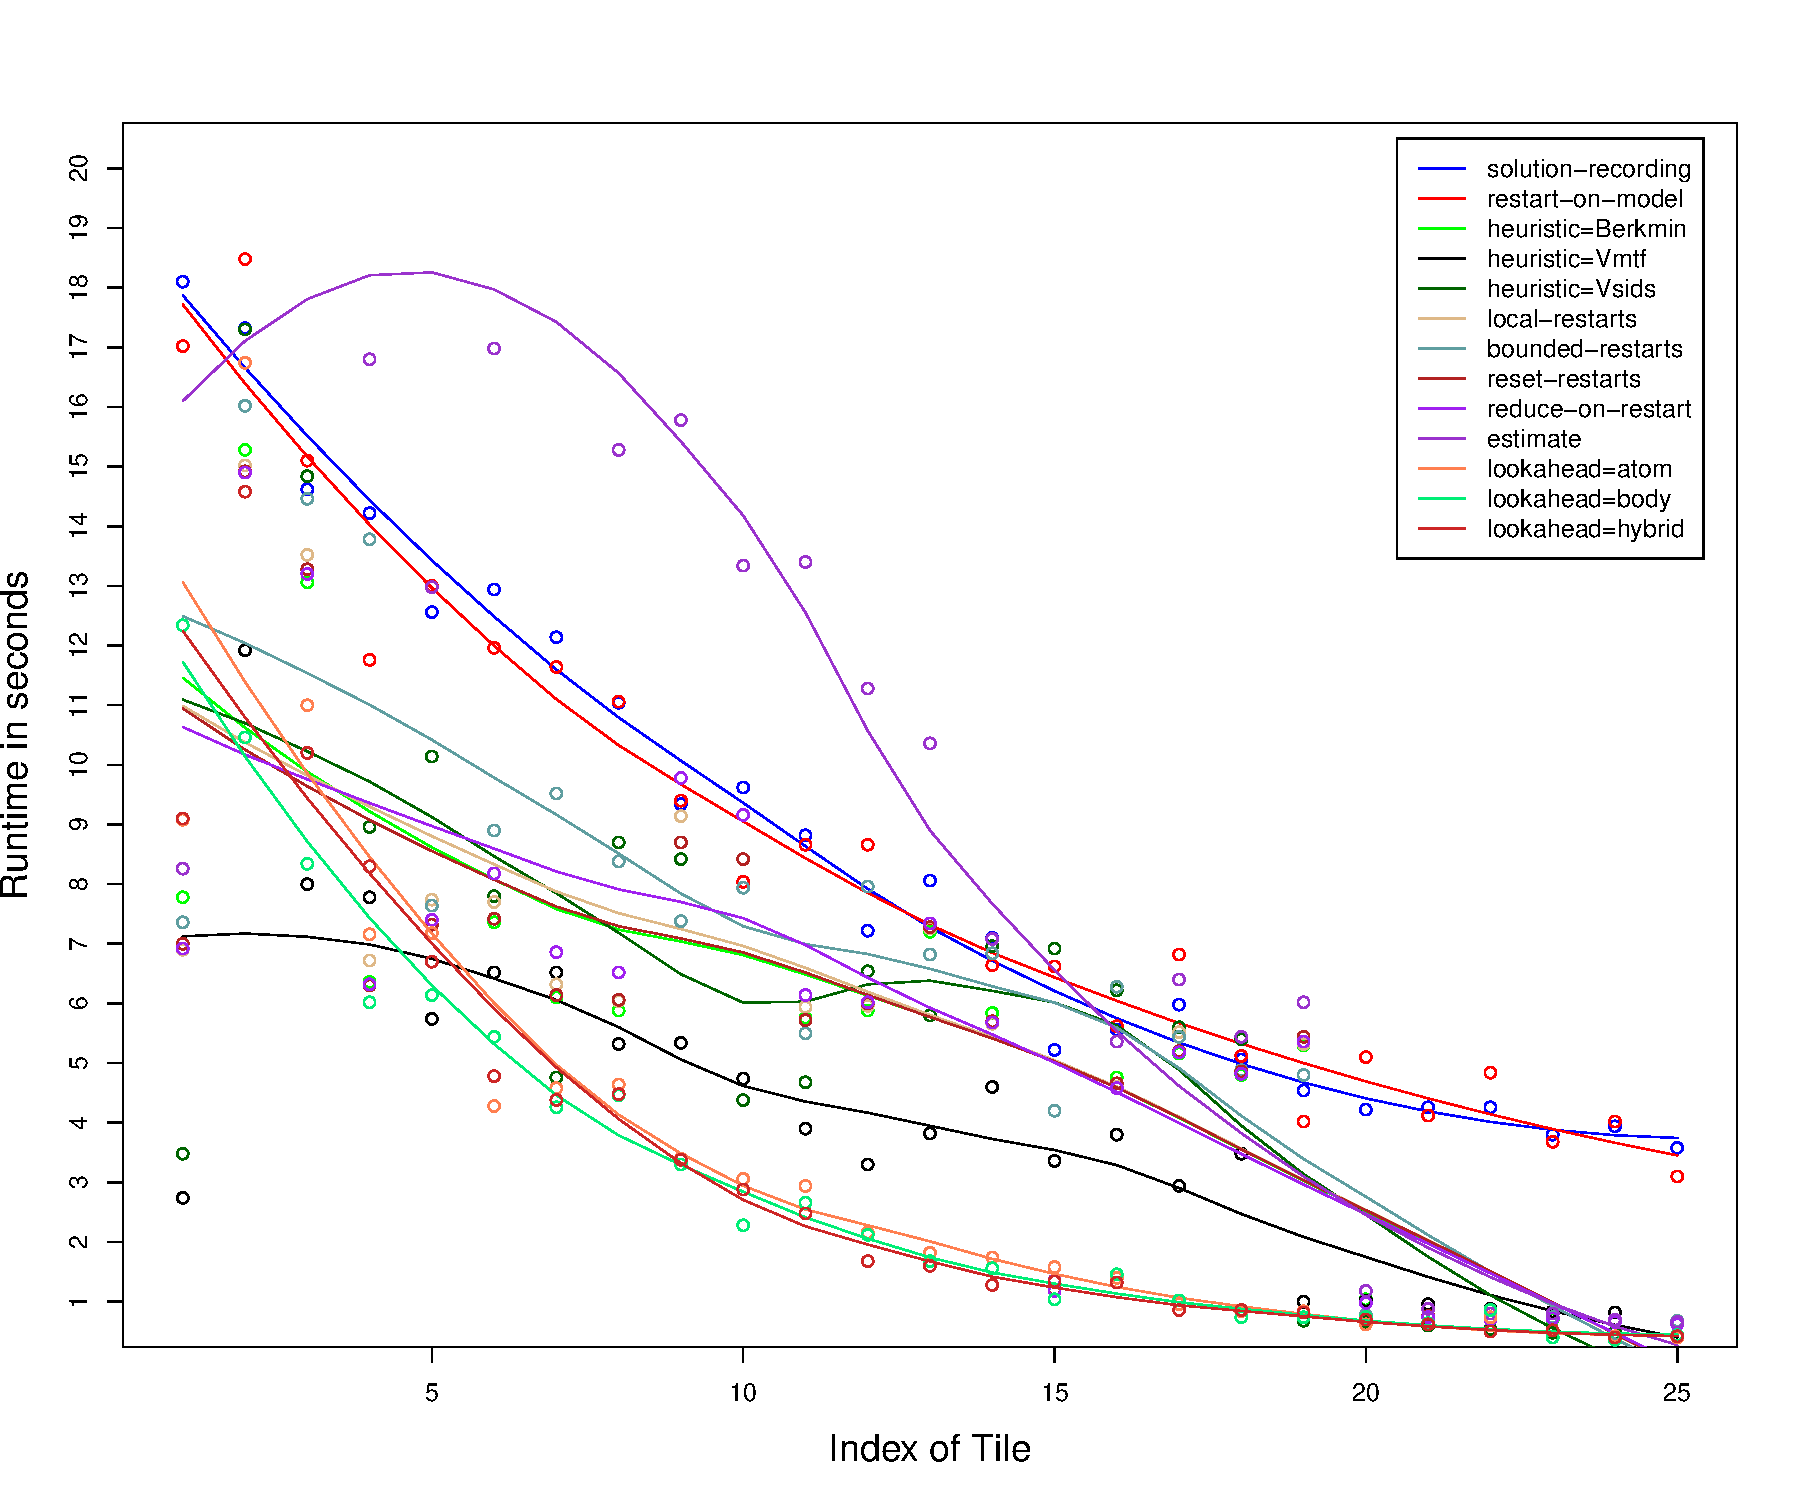
\includegraphics[width=1.12\textwidth]{time_parameters.pdf}
\end{subfigure}
   \hfill 
\begin{subfigure}{.47\textwidth}
  \caption{Runtime (in s) for $N$ tiles}
   \scalebox{.75}{
  \begin{tabular}{lrrrrr}
    \phantom{Search option} & \multicolumn{5}{c}{\textbf{Number of tiles}}\\
     \textbf{Search option} &  \textbf{5}     & \textbf{10}      &  \textbf{15}     &   \textbf{20}   &  \textbf{25}    \\
   \hline
  solution-recording  & 76  &131   & 168  & 193 &  213\\
  restart-on-model    & 75  &127   & 164  & 191 &  211\\
  heuristic=Berkmin   & 50  &86    & 112  & 133 &  137\\
  \textbf{heuristic=Vmtf}      & \textbf{36}  &\textbf{64}    & \textbf{83}   & \textbf{95}  &  \textbf{100}\\
  heuristic=Vsids     & 54  &88    & 119  & 138 &  140\\
  local-restarts      & 49  &87    & 113  & 134 &  138\\
  bounded-restarts    & 59  &101   & 132  & 154 &  158\\
  reset-restarts      & 48  &85    & 111  & 132 &  136\\
  reduce-on-restart   & 48  &89    & 115  & 136 &  139\\
  estimate            & 86  &169   & 213  & 237 &  241\\
  \textbf{lookahead=atom}    & \textbf{51} &\textbf{71}   & \textbf{81}  & \textbf{86} &  \textbf{88}\\
  \textbf{lookahead=body}    & \textbf{43} &\textbf{63}   & \textbf{72}  & \textbf{76} &  \textbf{79}\\
  \textbf{lookahead=hybrid}  & \textbf{48} &\textbf{68}   & \textbf{77}  & \textbf{81} &  \textbf{84}\\
   \end{tabular}
}
\phantom{teeext}\\
\end{subfigure}
  \caption{Determining the best ASP solver parameters for tiling with the model of Listing~\ref{lst:encoding}: (a) the runtime (in s) needed for mining each subsequent individual tile, (b) runtime summary (in s) for first 25 tiles}
  \label{meta-time}
\end{center}
\end{figure}

This appendix briefly evaluates the performance of the solver that was used for the experiments. We first describe how we tuned the system and then continue with an analysis of the solving process.

\textit{Solver tuning.} The clingo system \citep{gebser2011potassco} has a variety of parameters that affect runtime. We performed a series of preliminary experiments to determine the parameters that were used for all other experiments in this section. These tuning experiments mostly concerned maximum $k$-tiling on datasets of moderate size, but some test experiments on other tasks did not reveal any discrepancies. 

Runtime was measured for a large number of search options while fixing the dataset and task. Figure~\ref{meta-time} shows the results obtained for maximum $k$-tiling on the Animals dataset. 
Search options ``heuristic=Vmtf'' and the ``lookahead'' options result in shorter runtimes, but the ``lookahead'' options do not scale well; with these options the system is unable to handle bigger datasets like Mushroom and Chess. Therefore, all remaining experiments in this section have been performed with ``heuristics=Vmtf''. None of the other combinations of parameters gave any substantial improvement in runtime.

\textit{Grounding-solving analysis} Besides measuring the time needed for the solver to provide an answer, it is also useful to look at the time needed for the individual execution steps. In case of answer set programming, solving a problem consists of two main steps: 1) grounding and 2) solving (or, alternatively, searching). 

Table~\ref{table:steps-time} presents results obtained for the maximum k-tiling problem, i.e., the time needed to compute a single tile, averaged over the first 15 tiles, split into grounding and solving time. For many ASP programs the grounding step is the bottleneck, but the results clearly demonstrate that this is not the case for our ReDF tasks: the ratio between solving and grounding time is generally large. (Due to long runtimes this experiment was not performed for Chess and Mushroom.)

The large ratios can be explained by the fact that we deal with optimization problems, as is usual in data mining. In the presence of an exponential number of answer sets and a binary predicate as the optimization criterion, it is natural to expect the solving part to be the computationally most intensive step. 

The results suggest that, if we would like to speed-up ReDF in ASP, we would have to focus on making the general solving process more efficient, possibly by using properties of the ReDF framework. Specialized mining algorithms, e.g., for tiling, demonstrate that faster solving is possible, but translating these efficient mechanisms to an ASP solver, which works completely differently, seems far from trivial.

\begin{table}\footnotesize
  \caption{Maximum k-tiling: grounding and solving -- avg time per tile (s), and their time ratio}
  \label{table:steps-time}
\vspace{-10pt}
\begin{center}
\begin{tabular}{lrrc}
  Dataset & Grounding & \phantom{text} Solving & \phantom{aaa} Ratio -- Solving/Grounding \\ \hline
Nursery     &2.173&38.185 & 18 \\
Voting      &0.052&8.350 & 161  \\
Animals     &0.020&2.728 & 136 \\
Tic-tac-toe &0.124&1.969 & 16  \\
Flare       &0.225&0.575 & 3
\end{tabular}
\end{center}
\end{table}

\textit{Alternatives to manual parameter tuning.} \textit{claspfolio} is a portfolio system for clasp \citep{gekakascsczi11a}. However, our experiments indicated that none of the precomputed models of claspfolio applied to the problems considered in this work and the system switches to the default solver. \textit{hclasp} \citep{conf/aaai/GebserKROSW13} introduces heuristics into the reasoning process of clasp. Since we consider a wide class of problems, it requires a nontrivial decision procedure to find the right heuristics for a particular task. We regard it as a possible direction for future research.

